As the invisible interface between the player's instructions window and the actor's execution logic, the Interpreter's responsibilities are considerably abstracted from normal gameplay programming. More specifically, the Interpreter is responsible for defining the game's assembly-like language, extracting player instructions from the user interface, and marshaling the release of commands to the actor for execution.

\subsubsection{Language}
The interpreter is responsible

\begin{itemize}
    \item INPUT
    
    The INPUT command instructs Computron to approach the puzzle's Input Box and retrieve the next value. If Computron is currently holding a value, he will discard it. If the Input Box is empty, Computron will retrieve and hold a NULL value.

    \item OUTPUT
    
    The OUTPUT command instructs Computron to approach the puzzle's Output Box and deposit his current value. If Computron is not holding anything, this instruction will be considered invalid and raise a runtime error. Otherwise Computron will deposit the value in the output box.

    \item JUMP
    
    The plain JUMP command instructs the interpreter to unconditionally move the program counter to a new line in the player's solution. This instruction has no effect on Computron.

    \item JUMP IF NULL
    
    The JUMP IF NULL is a conditional jump instruction, which is only activated if the Actor is not holding any value. This instruction is often used to break out of loops.

    \item JUMP IF LESS [X]
    
    The JUMP IF LESS [X] is a conditional jump instruction, which is only activated if the Actor the value the actor is holding is less than the value stored in player-specified register X. If register X is empty, this instruction will be considered invalid and raise a runtime error.

    \item JUMP IF GREATER [X]
    
    The JUMP IF GREATER [X] is a conditional jump instruction, which is only activated if the Actor the value the actor is holding is greater than the value stored in player-specified register X. If register X is empty, this instruction will be considered invalid and raise a runtime error.

    \item MOVETO [X]
    
    The MOVETO [X] command instructs Computron to move the value currently being held into the player-specified register X. If Computron's hands are currently empty, this instruction will be considered invalid and raise a runtime error. If there is a value currently in the register, it will be overwritten.

    \item MOVEFROM [X]
    
    The MOVEFROM [X] command instructs Computron to remove the value currently being stored in in the player-specified register X. If the register is empty, Computron will retrieve and hold a NULL value. If Computron is currently holding a value, it will be overwritten.

    \item COPYTO [X]
    
    The COPYTO [X] command instructs Computron to move the value currently being held into the player-specified register X. Computron will retain a copy of the number. If Computron's hands are currently empty, this instruction will be considered invalid and raise a runtime error. If there is a value currently in the register, it will be overwritten.

    \item COPYFROM [X]
    
    The COPYFROM [X] command instructs Computron to retrieve a copy of the value currently being stored in in the player-specified register X. If the register is empty, Computron will retrieve and hold a NULL value. If Computron is currently holding a value, it will be overwritten.

    \item ADD [X]
    
    The ADD [X] command instructs Computron to add the value stored in player-specified register X to the value currently held. If either Computron's hands or register X are empty, this instruction will be considered invalid and raise a runtime error. Otherwise, Computron will perform the addition and overwrite his current value.

    \item SUBTRACT [X]
    
    The SUBTRACT [X] command instructs Computron to subtract the value stored in player-specified register X to the value currently held. If either Computron's hands or register X are empty, this instruction will be considered invalid and raise a runtime error. Otherwise, Computron will perform the subtraction and overwrite his current value.
\end{itemize}

\subsubsection{Program Counter}
To facilitate proper simulation of the player's solution, the interpreter will need to maintain a program counter that iterates and jumps through the player's code appropriately. To ensure that these updates happen correctly, the Interpreter will need to rely on reports from the Actor that state the validity of instructions and the result of conditional expressions.

\subsubsection{UI Interface}
To fulfill its responsibilities, the Interpreter will need to communicate closely with the User Interface to retrieve player instructions and report the state of the program counter. Figure \ref{fig:interpreter_UI_interface} illustrates the nature of these interactions.

\begin{figure}[!hb]
    \caption{Interpreter/UI Interface Overview}
    \label{fig:interpreter_UI_interface}
    \centering
    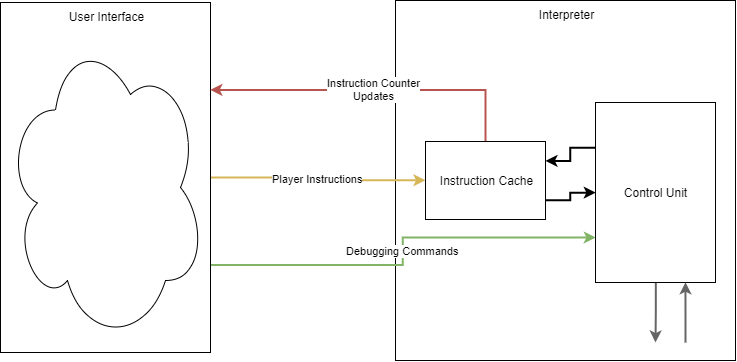
\includegraphics[width=\textwidth]{Diagrams/Interpreter_UI_Interface.png}
\end{figure}

\subsubsection{Actor Interface}
The Interpreter's Actor interface is responsible for making instructions available to the Actor on demand. In order to ensure the program counter is updated properly, the Interpreter and Actor engage in a 3-way handshake (shown in \ref{fig:interpreter_Actor_interface}). 

The stages of the handshake are:

\begin{figure}[!hb]
    \caption{Interpreter/UI Interface Overview}
    \label{fig:interpreter_Actor_interface}
    \centering
    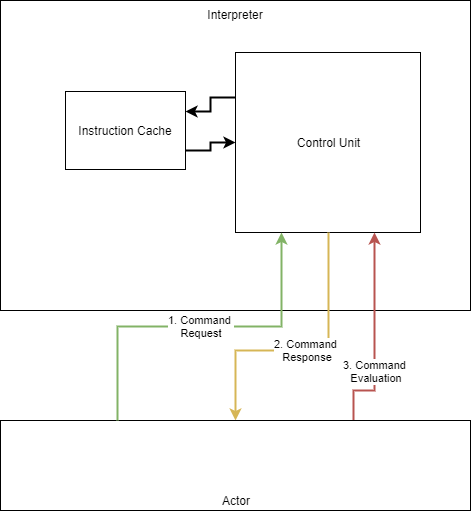
\includegraphics[width=\textwidth]{Diagrams/Interpreter_Actor_Interface.png}
\end{figure}

\begin{enumerate}
    \item Command Request
    
    The first step of the Actor control exchange is the Command Request. The actor will issue a Command Request to the interpreter when the next player instruction is needed.

    \item Command response
    
    The second step of the exchange is the Command Response. This response will be a data structure for the actor to parse, including the next instruction's opcode and argument.

    \item Command Evaluation
    
    The last step of the exchange is the Command Evaluation. This stage is the Actor's chance to report runtime errors to interpreter if the instruction is deemed invalid and report the result of a conditional expression if the instruction included one. 
\end{enumerate}